
\chapter{Algoritmos de Simulación}


\begin{figure}[H]
\centering
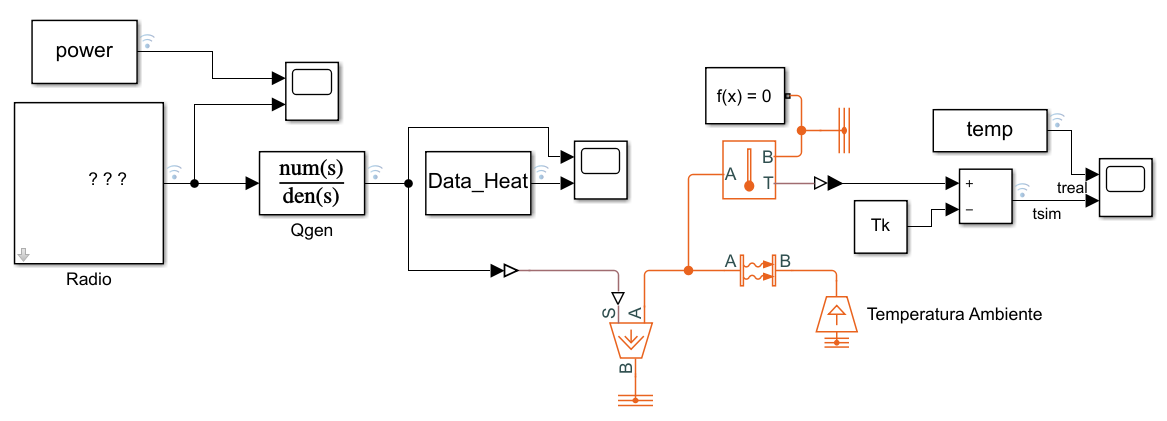
\includegraphics[scale=0.5]{Figuras/modelo_radio.png}
\caption{Algoritmo del modelo para el radio}
\centering
Fuente: Elaboración Propia
\label{anexo7}
\end{figure}

\begin{figure}[H]
\centering
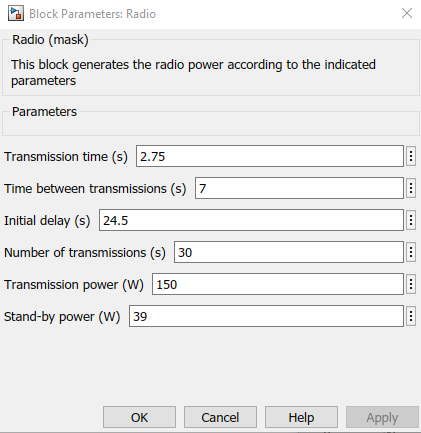
\includegraphics[scale=0.7]{Figuras/parametros_resultado.png}
\caption{Parámetros de entrada del modelo}
Fuente: Elaboración Propia
\label{anexo8}
\end{figure}


\begin{figure}[H]
\centering
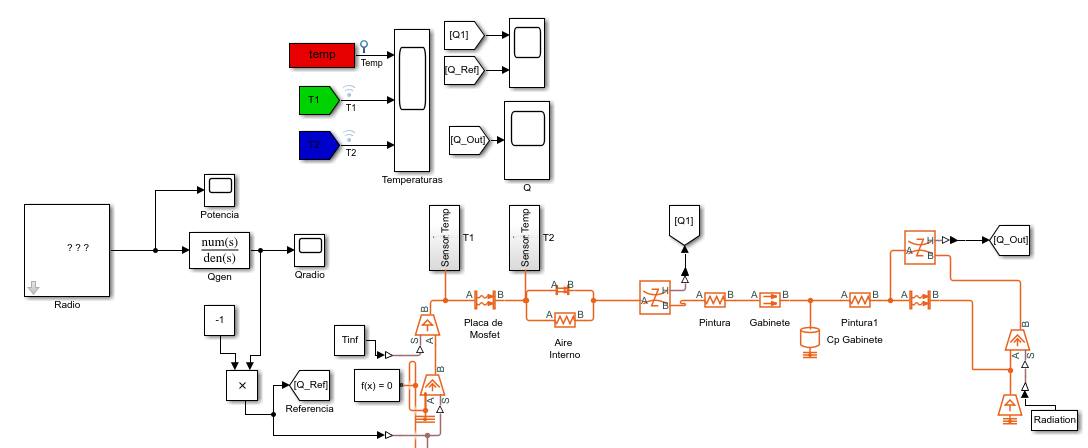
\includegraphics[width=\linewidth]{Figuras/Algoritmo_GTR.png} %nunca debe ser mas grande que los margenes, aqui mejor usar \linewidth
\caption{Algoritmo para la GRT}
Fuente: Elaboración Propia
\label{anexo10}
\end{figure}

\begin{figure}[H]
\centering
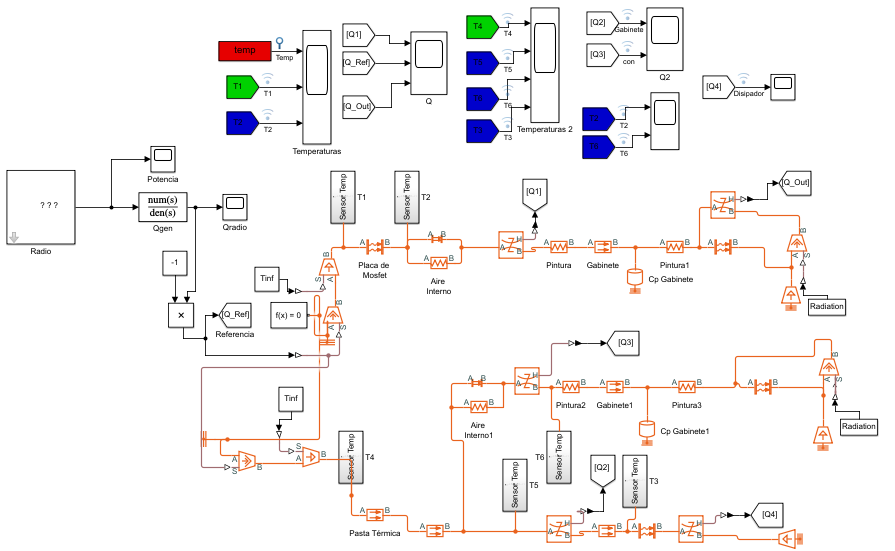
\includegraphics[scale=0.6]{Figuras/algoritmo_final.png}
\caption{Algoritmo con disipador de calor}
Fuente: Elaboración Propia
\label{anexo11}
\end{figure}